\chapter{Lexical Substitution}
\label{ch:lexsub}



\begin{comment}
  Outline
  - Chapter Summary
  - Introduction to Lexsub
  - Prior Work
  - Proposed model
  - Evaluation
  - Analysis
  - Chapter Summary
\end{comment}


This chapter shows new model of lexical substitution, and related
material. The work in this chapter has been published in
\newcite{roller:2016:naacl}.

\section{Chapter Overview}

Lexical substitution~\cite{mccarthy:2007:semeval} is a task in which word
meaning in context is described not through dictionary senses but through
substitutes (paraphrases) chosen by annotators.

\section{Lexical Substituion}

In our discussion of lexical relationships in the previous two chapters, we
assumed that words are {\em monosemous}, or that they have only one meaning.
However, words like \lit{bright} have multiple meanings, which change depending
on context, as in \lit{bright girl} and \lit{bright coat}. When a word has
multiple meanings, it is {\em polysemous}, and polysemy is yet another source
of ambiguity in natural language.

One issue with polysemy is what representation should even be chosen to
represent a polysemous word?  One option is the use of a lexicon, like the
dictionary.  Lexicographers are responsible for cataloguing and defining word
senses; one may see this in the multiple definitions provided by the Oxford
English Dictionary or Merriam Webster, but even professional lexicographers
often disagree on how many senses a word has. For example, \lit{bank} has
three noun senses in Webster's dictionary, but only two in Oxford's.
WordNet \cite{miller:1995:acm} is one of the most popular and heavily used
computational dictionaries, and is notoriously fine-grained (it gives 10
noun senses for \lit{bank}).

Even after one fixes the inventory of word senses, labeling a particular
instance of a word with its sense is fraught with its own difficulties:
non-experts have very low inner annotator agreements \cite{yong:1999:siglex},
and even lexicographers will disagree often \cite{kilgarriff:2000:ch}.
Results in computational approaches to Word Sense Induction (WSI) and Word
Sense Disambiguation (WSD) reflect this task difficulty \cite{needcite}.

Distributional Semantics offers an alluring alternative path, given its ability
to measure the {\em graded} levels of similarity between words
\cite{erk:2008:emnlp}.  One possibility is the use of multiple vectors per word
or word sense \cite{reisinger:2010:naacl,huang:2012:acl}, and then using using
these prototypes appropriately for downstream tasks. If one takes this idea to
its absolute extreme, one can imagine a new vector for every instantiation of a
word. In this extreme, one may choose not to create a unique vector for every
word, but instead model how meaning {\em shifts} in a particular given context.

One way to measure this has been the Lexical Substitution task. In
the Lexical Substitution task, we are provided with a sentential context, and
must suggest {\em substitutes} which can replace the given target word, while
preserving the meaning of the entire sentence
\cite{mccarthy:2007:semeval,biemann:2012:lrec,kremer:2014:eacl}.
Sometimes only a small context is needed for the task, as in \lit{bright girl}
and \lit{bright lamp}, but humans are often particularly creative when
providing suggestions. In one data set, humans provided with the context
\begin{quote}
  ``Tara stood stock-still, waiting for the first tiny gleam from the
  scout craft to appear in the darkness of the {\bf wormhole},''
\end{quote}
human annotators considered {\em portal} and {\em rift} to be excellent
substitutes. These substitutes take into account the Science Fiction context of
the sentence, indicating the task is more complicated than simple synonymy.
Indeed, in one one lexical substitution dataset, only 9\% of substitutes in
their dataset were direct synonyms in WordNet \cite{kremer:2014:eacl}.

\section{Prior Work}

\begin{comment}
Unsupervised approaches:

\end{comment}

In general, the Lexical Substitution task has seen a smaller research
investment than task like identifying lexical relationships. Nonetheless, a
wide variety of approaches have been taken, especially using distributional
vectors.

The original SemEval shared task released a moderately sized dataset and
defined the task \cite{mccarthy:2007:semeval}. The experimental setup was
specifically designed in order to elicit responses to polysemy in human
annotators. The corpus collectors selected a set of 2211 sentences containing
a targeted list polysemous words curated both manually and automatically using
lexical resources. These words cover several part-of-speech tags, and sentences
were manually selected to prevent primary senses from dominating the corpus.
Five human annotators were then asked to propose substitutes for the target
words in the sentential context: phrases and moderate generalizations were
allowed, but discouraged. The unification of substitutions resulted in a ranked
list of substitutes for every sentential context. Shared task participants
were asked to perform the same task computationally: both suggesting and
ranking possible substitutes.

Performance for the task was measured in {\em precision out of ten} (oot),
where a system was able to make up to ten guesses and the average percentage
of correct guesses across all sentences was reported; and {\em best}, where
a system provided its single best substitute and evaluated on whether that
substitute was proposed by any annotator.

A clear majority of systems used some lexical resource, like WordNet, to first
provide a list of possible substitutions, and then filtered or ranked that list
using their own research methods. Several used a mixture of co-occurrences or
$n$-grams to find good matches, and several used distributional methods to rank
the substitutes, almost no systems used existing WSD datasets
\cite{mccarthy:2007:semeval}. The best performing system differed for the two
metrics, with the strongest team on the {\em best} metric used a
supervised approach where substitutes were ranked with a supervised model
using features like $n$-gram likelihood \cite{yuret:2007:semeval}. The strongest
performing system in {\em oot} beat the competition by a large margin, but
performed nearly last in the {\em best} metric.  Unfortunately, it turned out
this system accidentally exploited a flaw in the evaluation metric by
predicting the same substitute multiple times without penalty
\cite{giuliano:2007:semeval}. Perhaps as a result of this accident, the
literature has since varied substantially on experimental setup and evaluation
metrics. Nonetheless, the task provided an interesting test bed for a
variety approaches, including distributional approaches, language modeling
approaches, and some supervised approaches \cite{szarvas:2013:naacl}.

\subsection{Unsupervised approaches}

One major insight from the competition was the importance of syntagmatic fit in
lexical substitution with the success of $n$-gram based models.
\newcite{erk:2008:emnlp} proposed using a model of "inverse" selectional
preferences to compute a word vector {\em in context}, and applied this model
to the task of lexical substitution. Their key insight was to model a word in
context by averaging over other possible fillers for the same syntactic
contexts. For example, in \lit{the fielder {\em catches}}, they would consider
verbs which take \lit{fielder} in the subject position, and so on for other
syntactic roles. Their work also took evaluation of lexical substitution in a
different direction: rather than evaluate their system on the task of both
suggestion and ranking of substitutes as in SemEval, they separated these tasks
and proposed evaluating on only the task of predicting which substitutes are
best for a particular instance.

\newcite{thater:2009:ati,thater:2010:acl} expanded on the this idea of inverse
selection preferences by proposing a {\em second-order} distributional space,
where syntactic co-occurrences were modeled via a sparse tensor representation
similar to TypeDM \cite{baroni:2011:gems}, and using multiple folds over the
tensor to produce a unique vector for each word in context.
\newcite{thater:2011:ijcnlp} refine and simplify on this second-order view of
the previous models by proposing to re-weight a word's syntactic co-occurrences
based on their similarity to the present context.
This unsupervised, method remained one of strongest performing systems even when
applied to new data sets \cite{kremer:2014:eacl} and compared to some
supervised systems. Along a similar path, \newcite{melamud:2015:naacl} proposed
an alternative second order model based on using Google's web corpus of
5-grams.

\newcite{dinu:2010:emnlp} showed that latent-factor distributional models like
Latent Dirichlet Allocation \cite{blei:2003:jmlr} could allow for evaluating
the particular fit of a given substitute. They considered two latent
factorization models (LDA and NNMF) and showed that context could successfully
modulate over varying latent senses of a particular word in a bag-of-words
context. This insight in the power of low-rank factorizations later turns
out to be valuable in later lines of work \cite{melamud:2015:vsm,roller:2016:naacl}.

\newcite{vandecruys:2011:emnlp} observed that syntax-based distributional
models tend to provide the strongest results, yet individual examples in
lexical substitution data {\em should} require a wider understanding of the
context, like in the \lit{wormhole} example provided earlier. They proposed a
{\em joint} latent factorization model over both a wide bag-of-words
co-occurrences with the functional, syntactic context. Although this line of
work has not seen a large degree of follow up, the author of this dissertation
hopes future research will reconsider this path.

More recently, some models have wielded the deep learning hammer for the task
of lexical substitution. \newcite{kawakami:2016:iclr} propose using word
alignments from translation tasks in order to identify the different senses of
a word in the hidden state of a bidirectional RNN. The intuition is that two
tokens which translate into the same foreign token have the same underlying
sense, while two tokens which translate into different foreign tokens must
represent a polysemous term, an idea has a long history in the literature
\cite{resnik:1999:nle,diab:2003:phd,bannard:2005:acl}. Since their model
requires substantial aligned translation corpora, it is not directly comparable
to the other models exploring the task. Therefore \newcite{melamud:2016:conll}
applied the same neural architecture, trained on an English-only language
modeling task, to lexical substitution, but found it still did not outperform
other models.

\subsection{Supervised approaches}

Another vein of research has treated Lexical Substitution as a truly
supervised research problem, as opposed to the predominantly unsupervised or
knowledge-transfer approaches listed above. For example, the original SemEval
task tuned a threshold on likelihoods obtained from a language
model \cite{yuret:2007:semeval}. Others have proposed more sophisticated
architectures based on producing context features for the target token
\cite{biemann:2012:lrec}, or a fully delexicalized classifier which learns over
features extracted via a (target, substitute) pair \cite{szarvas:2013:naacl}.
Another approach from \newcite{szarvas:2013:emnlp} notes that previous
approaches emphasize the importance of ranking properly, and proposes to treat
lexical substitution as a true ranking problem. This substantially outperforms
the other ranking approaches, but the comparison is unfair due to differing
levels of supervision.

One important model in the context of our own work is the extremely simple,
yet high-performing method by \newcite{melamud:2015:vsm}. They propose using
the {\em context vectors} from a syntactic word2vec model \cite{levy:2014:acl}
in to compute a score for 


Recent models include a simple but high-performing method by Melamud et
al.~\shortcite{melamud:2015:vsm}, which uses the Skip-gram model of Mikolov et
al.~\cite{mikolov:2013:iclr} to compute the probability of a substitute given a
sentence context, and integrates it with the probability of the substitute
given the target. The current state of the art is held by another model of
Melamud ~\cite{melamud:2015:naacl}, which uses a more complex architecture.
%Curiously, most models for lexical substitution so far have been unsupervised,
and the supervised de-lexicalized model of Szarvas et
al.~\shortcite{szarvas:2013:naacl} is not superior to current unsupervised
approaches. 



\section{Probability-in-Context (PiC)}

We build on the simple model of Melamud et al.~\shortcite{melamud:2015:vsm}, as
simpler methods are easier to recreate and integrate into larger pipelines. We
explore a weak form of supervision that recently has proved beneficial on many
NLP tasks: using a language modeling task on unannotated data.


We propose a new measure, which extends
a previously successful, simple model to estimate the appropriateness of a
lexical substitute. As a introduction point for our measure, we review the work
of \newcite{melamud:2015:vsm}, which introduced several unsupervised measures
for word similarity in context: namely \balAddCos and \addCos. The main insight
of these unsupervised measures is the use of {\em context vectors}, related
to the insights discussed in Section~\ref{sec:lexmem}. Crucially, the models
of \newcite{melamud:2015:vsm} depend on syntactic context vectors, which
have been found more successful than just BoW measures in the literature
\cite{erk:2008:emnlp,dinu:2010:emnlp,thater:2010:acl,vandecruys:2011:emnlp}.
We note that these models are {\em not} the state of the art,
\cite{melamud:2015:naacl,melamud:2016:conll} but perform competitively while
remaining simple, extensible, and highly interpretable.

In the work of \newcite{melamud:2015:vsm} and others, substitutes are modeled
using a mixture of {\em out-of-context similarity} and {\em in-context
appropriateness}. The out-of-context similarity uses standard distributional
semantics cosine similarity (Equation~\ref{eq:cos}) in order to estimate how similar
the target is to the substitute, and remains fixed regardless of the sentential
context.  For this reason, this out-of-context (OOC) similarity is also used as
a baseline in the literature.

The in-context appropriateness attempts to directly model
whether a proposed substitute fits in the given sentential context. That is, if
one replaces the target with the substitute directly, would a reader still
consider this word {\em selectionally} agrees in the sentence. For example,
the in-context measures will give a low score for {\em dog purrs}, since dogs
usually do not purr.
To this end, it assumes the sentence is parsed, so that we have the full set of
syntactic neighbors of the target, $C$. Each of the context vectors
corresponding to elements of $C$ are then evaluated for their fit with the
proposed substitute, as illustrated in Figure~\ref{fig:syn}. For a given target
$t$, substitute $s$ and context $C$, the final \addCos~score is given as
\begin{equation}
  \text{addCos}(s|t,C) = \text{cosine}(s, t) + \sum_{c\in C} \text{cosine}(s, c).
\end{equation}
The model can be intuitively understood using the diagram in
Figure~\ref{fig:substitution}. For a given target ``bright,'' we will choose
the substitute (``smart'' or ``colorful'') which is {\em closer} to the
given context. If the context is ``scientist'' as in ``bright scientist,''
we will shift our prediction away from ``colorful'' and closer to ``smart,''
and vice versa for ``bright coat.'' This remains one of the simplest successful
models of Lexical Substitution to date. \newcite{melamud:2015:vsm} also consider
variants of this measure, including {\em balAddCos}, which equally
weights the out-of-context similarity with the in-context appropriateness:
\begin{equation}
  \text{balAddCos}(s|t,C) = \text{cosine}(s, t) + \frac{1}{|C|}\sum_{c\in C} \text{cosine}(s, c).
\end{equation}

In our work, we propose a new measure, called Probability-in-Context (PIC),\footnote{PIC is not strictly a probability measure; the name is a backronym for the purpose of the paper's title.}
which estimates the appropriateness of a substitute in a given context
\cite{roller:2016:naacl}.  Similar to \balAddCos, the measure has two
equally-weighted, independent components measuring the appropriateness of the
substitute for both the target and the context, each taking the form of a
softmax:
\begin{equation}
  \begin{aligned}
  \mbox{PIC}(s | t, C) &\propto P(s | t) \times P(s | C)\\
  P(s | t) &= \frac{1}{Z_t}\exp\left\{s^\top t\right\}\\
  P(s | C) &= \frac{1}{Z_C}\exp\left\{\sum_{c\in C}s^\top\left[Wc + b\right]\right\},
  \end{aligned}
  \label{eqn:pic}
\end{equation}
where the $Z_t$ and $Z_C$ are normalizing constants.
Our model differs from {\em balAddCos} in one major way: we base our similarity
estimates using the {\em unnormalized} inner product $s^\top t$ and $s^\top c$,
rather than normalized cosine similarities. We also introduce two additional
parameters, $W$ and $b$, which act as a simple linear transformation over the
original context vectors. These parameters are learned from the original
corpus, and serve only to tune how the fixed distributional vectors act in this
alternative objective function.

To identify the contribution of this parameterization versus the softmax
objective, we also introduce to a non-parameterized PIC ({\em nPIC}), which
does not contain the extra parameters:
\begin{equation}
  \begin{aligned}
  \mbox{nPIC}(s | t, C) &= P(s | t) \times P_n(s | C)\\
  P_n(s | C) &= \frac{1}{Z_n}\exp\left\{\sum_{c\in C}s^\top c\right\}
  \end{aligned}
  \label{eqn:npic}
\end{equation}

We compare our model to that of an out-of-context baseline (cosine) and the
{\em addCos} and {\em balAddCos} models of \newcite{melamud:2015:vsm}, which
outperformed other prior work at the time of its publication. We compare the
models on three data sets: SE07, the original LexSub data set
\cite{mccarthy:2007:semeval} which was explicitly developed to capture polysemy;
Coinco, a recent LexSub data set which contains substitutes for all content
words in a small corpus \cite{kremer:2014:eacl}; and TWSI2, which was developed
to be a large collection of lexical substitutes from a diverse corpus
\cite{biemann:2012:lrec}. We measure performance in Mean Precision@1, which
measures whether our best proposed substitute is contained within the set of gold
substitutes provided by annotators. In all models, we exclude any words sharing
the same lemma as the target, e.g. if the target is ``barking'' we do not
propose ``bark.''


\hardline

We propose a new measure, called Probability-in-Context (PIC), based
on SGNS context vectors to estimate the appropriateness
of a lexical substitute. Similar to \balAddCos, the measure has two equally-weighted,
independent components measuring the appropriateness of the substitute
for both the target and the context, each taking the form of a
softmax:\footnote{Note that $P(s|t)$ measures paradigmatic similarity
  of $s$ and $t$, while $P(s|C)$ is syntagmatic fit to the
  context.
  %Both take the same shape of a dot product.
  For $P(s|t)$,
  Mikolov et al.~\shortcite{mikolov:2013:iclr} show that cosine
  similarity of SGNS embeddings predicts
  paradigmatic similarity. $P(s|C)$ can be interpreted as the PMI of
  $s$ and $C$~\cite{levy:2014:nips}.}
\begin{align*}
  \mbox{PIC}(s | t, C) &= P(s | t) \times P(s | C)\\
  P(s | t) &= \frac{1}{Z_t}\exp\left\{s^\top t\right\}\\ %{\sum_{s'}\exp\left\{s'\cdot t\right\}}
  P(s | C) &= \frac{1}{Z_C}\exp\left\{\sum_{c\in C}s^\top\left[Wc + b\right]\right\}
\end{align*}

The values $Z_t$ and $Z_C$ are normalizing constants to make sure each
distribution sums to one. This measure has two free parameters, $W$ and $b$,
which act as a linear transformation over the context vectors. These parameters
are estimated from the {\em original corpus}, and are trained to maximize
the prediction of a {\em target} from only its syntactic contexts (c.f. Section~\ref{sec:training}).
Given this formulation, a natural question is why not train the embeddings to optimize the
softmax directly? We choose to parameterize the measure rather than the
embeddings because (i) SGNS embeddings are already popular and readily
available and
(ii) it ensures the quality of embeddings remains constant across experimental 
settings.

To measure the importance of parameterization, we
also compare to a non-parameterized PIC (\ourmeas), which only uses a softmax over the
dot product:
\begin{align*}
  \mbox{nPIC}(s | t, C) &= P(s | t) \times P_n(s | C)\\
  P_n(s | C) &= \frac{1}{Z_n}\exp\left\{\sum_{c\in C}s^\top c\right\} %{\sum_{s'}\exp\left\{\sum_{c\in C}{s'\cdot c}\right\}}
\end{align*}

%\red{Need something else to close this section, Katrin?}
%Both of these proposed measures rely on the same intuitions and context
%embeddings as \balAddCos, can be implemented just as easily, but per
%

\begin{figure}
\centering
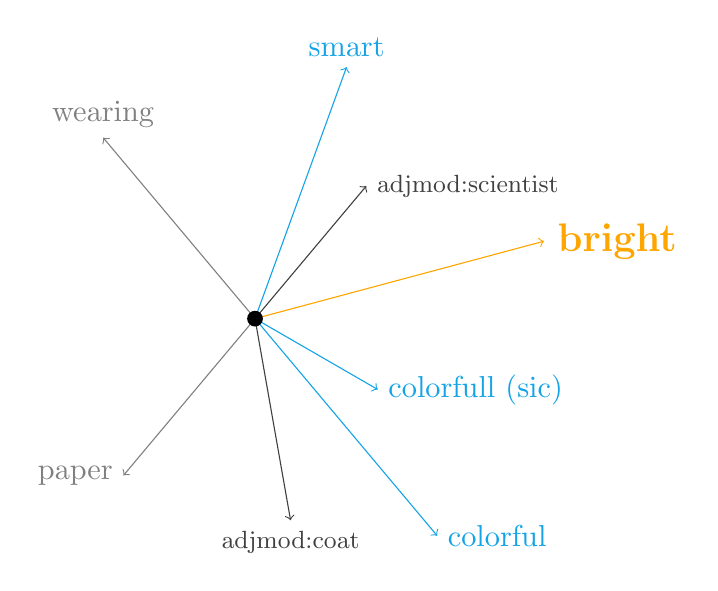
\begin{tikzpicture}[scale=2.0]
    \fontsize{11}{11}\selectfont
    \coordinate (origin) at (0,0);
    \draw [->,Gray] (origin) -- (130:1.5) node[above] {{wearing}};
    \draw [->,Gray] (origin) -- (230:1.3) node[left] {{paper}};
    \draw [->,Cerulean] (origin) -- (310:1.8) node[right] {{colorful}};
    \draw [->,Cerulean] (origin) -- (330:0.9) node[right] {{colorfull} (sic)};
    \draw [->,Cerulean] (origin) -- (70:1.7) node[above] {{smart}};
    \draw [->,darkgray] (origin) -- (280:1.3) node[below] {{\small \ctx{adjmod\depinv:coat}}};
    \draw [->,darkgray] (origin) -- (50:1.1) node[right] {{\small \ctx{adjmod\depinv:scientist}}};
    \fontsize{14}{14}\selectfont
    \draw [->,Orange] (origin) -- (15:1.9) node[right] {\bf{bright}};
    \fill (origin) circle (0.05);
\end{tikzpicture}
\caption{Cartoon illustration of how context vectors can disambiguate word senses.}
\label{fig:substitution}
\end{figure}


\section{Experiments and Results}
We compare our proposed measures to three baselines: \ooc, the Out-of-Context
cosine similarity between the word and target ($\mbox{cos}(s, t)$), and the \addCos~and \balAddCos~
measures. It is important to note that existing papers on Lexical Substitution all contain subtle
differences in experimental setup (vocabulary coverage, candidate pooling,
etc.). We compare to our own re-implementation of the baselines, so our
numbers differ slightly from those in the literature.

\subsection{Data sets}

We evaluate on three lexical substitution data sets.

{\bf SE07}: The data set used in the original SemEval 2007 shared task \cite{mccarthy:2007:semeval}
consists of 201 words manually chosen to exhibit polysemy, with 10 sentences
per target. For a given target in a particular context, five annotators were asked to propose up
to 3 substitutes. As all our experiments are
unsupervised, we always evaluate over the entire data set, rather than the
original held-out test set.

{\bf Coinco}: The Concepts-in-Context data set \cite{kremer:2014:eacl} is a large
lexical substitution corpus with proposed substitutes for nearly all content
words in roughly 2,500 sentences from a mixture of genres (newswire, emails,
and fiction). Crowdsourcing was used to obtain a minimum of 6
contextually-appropriate substitutes for over 15k tokens.
%The data set was {\em not} constructed specifically to capture polysemy, but does. 

{\bf TSWI2}: The Turk bootstrap Word Sense Inventory 2.0 \cite{biemann:2012:lrec}
is a crowdsourced lexical substitution corpus focused on about 1,000 common
English nouns. The data set contains nearly 25,000 contextual uses of these
nouns. Though the data set was originally constructed to induce a word-sense
lexicon based on common substitution patterns, here we only use it as a
lexical substitution data set.

\subsection{Task Evaluation}

We compare models on two variations of the lexical substitution task: candidate
ranking and all-words ranking. In the {\em candidate ranking} task, the model is
given a list of candidates and must select which are most appropriate
for the given target. We follow prior work in pooling candidates from all
substitutions for a given lemma and POS over all contexts, and measure
performance using Generalized Average Precision (GAP).  GAP is similar to Mean
Average Precision, but weighted by the number of times a substitute was given
by annotators.  See \newcite{thater:2010:acl} for full details of the
candidate ranking task.

The second task is the much more difficult %, but realistic 
task of {\em all-words
ranking}.  In this task, the model is not provided any gold list of candidates,
but must select possible substitutes from the entire vocabulary.\footnote{All models are also hardcoded not to predict substitutes
with the same stem as the target, e.g. for the {\em bright girl} example, models cannot predict {\em brighter} or {\em brightest}.}
We measure performance by (micro) mean Precision@1 and P@3: that is, of a system's top
one/three guesses, the percentage also given by human annotators.  These
evaluation metrics are similar to the {\em best} and {\em oot} metrics
reported in the literature, but we find P@1 and P@3 easier to interpret and
analyze.

\subsection{Word and Context Vectors}

We use the word and context vectors released by
\newcite{melamud:2015:vsm},\footnote{\url{http://www.cs.biu.ac.il/nlp/resources/downloads/lexsub_embeddings}}
which were previously shown to perform strongly in lexical substitution
tasks. These embeddings were computed from a corpus of
(word, relation, context) tuples extracted from ukWaC and processed using the
dependency-based word2vec model of \newcite{levy:2014:acl}. These embeddings
contain 600d vectors for 173k words and about 1M syntactic contexts.


\subsection{Training Procedure}
\label{sec:training}

To train the $W$ and $b$ parameters, we extract tokens with syntactic contexts
using the same corpus (ukWaC), parser \cite{chen:2014:emnlp}, and extraction procedure
used to generate the embeddings. See \cite{melamud:2015:vsm} for complete details.
After extracting every token with its contexts, we randomly sample 10\% of the
data to reduce computation time, leaving us with 190M tokens for training $W$ and $b$.
We use sampled softmax to reduce training time \cite{jean:2015:acl},
sampling 15 negative candidates uniformly from the vocabulary, optimizing
cross-entropy over just these 16 words per sample.
We optimize $W$ and $b$ in one epoch of stochastic gradient descent (SGD) with
a learning rate of 0.01, momentum of 0.98, and a batch size of 2048. We found
all of these hyperparameters worked well initially, and did not tune them.
% This procedure took around 45 minutes using a GPU.


\subsection{Results}
\begin{table}
\centering
\begin{tabular}{|lccc|}
  \hline
  {\bf Measure} & {\bf SE} & {\bf CiCo} & {\bf TWSI}\\
  \hline\hline
  \ooc               &     44.2   &     44.5  &     57.9       \\
  \addCos            &     51.2   &     46.3  &     62.2       \\
  \balAddCos         &     49.6   &     46.5  &     61.3       \\
  \hline
  \ourmeas           &     51.3   &     46.4  &     61.8       \\
  \ourmeasparam      & {\bf52.4}  & {\bf48.3} & {\bf62.8}      \\
  \hline
\end{tabular}
\caption{Performance of {\ourmeas} and {\ourmeasparam} on the three Lexical
  Substitution datasets in the all candidate ranking task, measured in GAP.}
\label{tab:precision}
\end{table}

\begin{table}
\centering
\begin{minipage}{6cm}
\centering
\begin{tabular}{|lccc|}
  \hline
  {\bf Measure} & {\bf SE} & {\bf CiC} & {\bf TWSI}\\
  \hline\hline
  \ooc               &     11.7   &    10.9   &      9.8       \\
  \addCos            &     12.9   &    10.5   &      7.9       \\
  \balAddCos         &     13.4   &    11.8   &      9.8       \\
  \hline
  \ourmeas           &     17.3   &    16.3   &     11.1       \\
  \ourmeasparam      & {\bf19.7}  &{\bf18.2}  & {\bf13.7}      \\
  \hline
\end{tabular}\\~\\(a) Precision@1
\end{minipage}
\quad
\begin{minipage}{6cm}
\centering
\begin{tabular}{|lccc|}
  \hline
  {\bf Measure} & {\bf SE} & {\bf CiC} & {\bf TWSI}\\
  \hline\hline
  \ooc               &     9.7    &     8.6   &     7.0       \\
  \addCos            &     9.0    &     7.9   &     6.1       \\
  \balAddCos         &     9.8    &     9.1   &     7.4       \\
  \hline
  \ourmeas           &    13.1    &    12.1   &     7.9       \\
  \ourmeasparam      &{\bf14.8}   &{\bf13.8}  &{\bf10.1}      \\
  \hline
\end{tabular}\\~\\(b) Precision@3
\end{minipage}
\caption{Performance of {\ourmeas} and {\ourmeasparam} on the three Lexical
  Substitution datasets in the all words ranking task, measured in
  (a)~Precision@1 and (b)~Precision@3.}
\label{tab:precision}
\end{table}

\hardline

Table~\ref{tab:lexsub} contains results for all measures across all datasets.
We observe that PIC outperforms all other models by a significant
margin,\footnote{Wilcoxon signed-rank test, $p < 0.01$} including a relative
30\% improvement over \balAddCos in SE07 and Coinco. The nPIC also improves
substantially over the other baselines, indicating we gain benefit both from
the new objective function and the additional parameterization.  We next
strive to understand why both measures have a clear improvements over the
baseline models.

\hardline

Table~\ref{tab:precision} contains results for all measures across all
experimental settings.

The first observation we make is that the \ourmeasparam~measure performs best
in all evaluations on all data sets by a significant margin.\footnote{Wilcoxon signed-rank test, $p < 0.01$}
In the GAP evaluation, all measures
perform substantially better than the \ooc~baseline, and the \ourmeas~measure
performs comparably to \balAddCos. We note that context-sensitive
measures give the most improvement in SE07, reflecting its greater emphasis on
polysemy.

As we turn to the all-words ranking evaluations, we observe that the absolute numbers are
much lower, reflecting the increased difficulty of the task. We also see the
that \ourmeas~and \ourmeasparam~both improve greatly over all baselines: The
\ourmeas~measure is a relative 30\% improvement over \balAddCos~in SE07 and
Coinco, and the \ourmeasparam~measure is a relative 50\% improvement over
\balAddCos~in 5 evaluations.

Since both measures have a clear improvement over the baselines, especially in
the more difficult all-words task, we next strive to understand why.


\subsection{Analysis}
\label{sec:lexsubanalysis}
\begin{table*}[t]
  \begin{center}
  \begin{tabular}{|cccc|}
    \hline
    \ooc             & \balAddCos            & \ourmeas         & \ourmeasparam\\
    \hline\hline
    \multicolumn{4}{|c|}{You can sort of challenge them well, did you}\\
    \multicolumn{4}{|c|}{{\bf really} know the time when you said yes?}\\
    \hline
    {    trully              } & {    proably             } & {    realy               } & {\bf actually            } \\
    {\bf actually            } & {    trully              } & {\bf truly               } & {\bf truly               } \\
    {    actaully            } & {    acutally            } & {\bf actually            } & {    already             } \\
    {    acutally            } & {    actaully            } & {    hardly              } & {    barely              } \\
    {    proably             } & {    probaly             } & {\bf definitely          } & {    just                } \\
    \hline
  \end{tabular}
  \end{center}
  \caption{Example where the \ourmeasparam~performs better in the All-Words Ranking task. The target word and correct answers
  are bolded.}
  \label{tab:cherry}
\end{table*}

\begin{table*}[t]
  \begin{center}
  \begin{tabular}{|cccc|}
    \hline
    {    OOC                 } & {    \balAddCos          } & {    \ourmeas            } & {    \ourmeasparam       } \\
    \hline\hline
    \multicolumn{4}{|c|}{As a general rule, point of view should not {\bf change} during a scene.}\\
    \hline
    {    sea-change          } & {\bf alter               } & {    reoccur             } & {    re-occur            } \\
    {\bf alter               } & {    sea-change          } & {    re-occur            } & {    appear              } \\
    {\bf shift               } & {\bf shift               } & {    prevail             } & {    overstate           } \\
    {    downshift           } & {    downshift           } & {    deviate             } & {    differ              } \\
    {    re-configure        } & {    increase/decrease   } & {    divulged            } & {    disappear           } \\
    %\hline\hline
    %\multicolumn{4}{|c|}{The cabin crew are {\bf rude} and unprofessional and seem}\\
    %\multicolumn{4}{|c|}{to treat the paying passenger as an unwelcome burden.}\\
    %\hline
    %{\bf impolite            } & {\bf impolite            } & {    polite              } & {    polite              } \\
    %{    discourteous        } & {    polite              } & {    unprofessional      } & {\bf impolite            } \\
    %{\bf disrespectful       } & {    discourteous        } & {    arrogant            } & {    inconsiderate       } \\
    %{    polite              } & {\bf disrespectful       } & {\bf impolite            } & {    arrogant            } \\
    %{    bitchy              } & {    bitchy              } & {\bf disrespectful       } & {\bf unkind              } \\
\hline
  \end{tabular}
  \end{center}
  \caption{Example where the \ourmeasparam~performs worse the All-Words Ranking task. The target word and correct answers
  are bolded.}
  \label{tab:lemon}
\end{table*}

We first examine cherry and lemon-picked examples to give intuitions about why
our model performs better. Table~\ref{tab:cherry} contains the cherry example,
where our model performs better than prior work. While OOC
and \balAddCos~both suggest replacements with reasonable semantics, but are
all misspelled. \ourmeas~and \ourmeasparam~only pick words with the correct spellings,
with the exception of ``realy.''

Table~\ref{tab:lemon} shows the lemon example, where our model performs worse.
We notice that the unusual ``sea-change'' item is prominent in the OOC and
\balAddCos~models, but has dropped from the rankings in our models. From
these and other examples, we hypothesize the model is simply guessing more
frequent terms.

\hardline

We characterize the models using a cherry-picked example,
given in Table~\ref{tab:cherry}. Although this example does not perfectly illustrate
the Lexical Substitution task, it does well at giving intuition as to why our
models perform better. We see that all four measures
tend to pick excellent substitutes which {\em semantically} agree with the
original target. However, the cosine and {\em balAddCos} models have a large number of
misspelled works in their list, while the nPIC and PIC measures contain
mostly correct spellings. This is because, somewhat surprisingly, the {\em
length} of the distributional vectors correlates strongly with the {\em
unigram} statistics of the word \cite{wilson:2015:arxiv}.
Therefore, by using the unnormalized inner
product, rather than cosine, our model naturally incorporates unigram priors,
allowing it to downweight rare, similar words. Indeed, a quantitative analysis
of the $W$ and $b$ parameters finds that they additionally exaggerate this
unigram bias \cite{roller:2016:naacl}.
Intuitively, it seems natural that unigram biases should hold a strong role in
Lexical Substitution, and that our model should wish to exploit this
information.


\hardline



We consider a few experiments with this hypothesis that the measures do better
because they capture better {\em unigram} statistics than the baselines. Recent literature found that the vector
norm of SGNS embeddings correlates strongly with word frequency
\cite{wilson:2015:arxiv}. We verified this for ourselves, computing the Spearman's
rank correlation between the corpus unigram frequency and the vector length
and found $\rho = 0.90$, indicating the two correlate very strongly. Since the
dot product is also the unnormalized cosine, it follows that \ourmeas~and
\ourmeasparam~should depend on unigram frequency.

To verify that the \ourmeas~and \ourmeasparam~measures are indeed preferring more frequent
substitutes, we compare the single best predictions (P@1) of the \balAddCos~and
\ourmeas~systems on all-words prediction on Coinco. Roughly 42\% of the predictions made
by the systems are identical, but of the remaining items, 74\% of
predictions made by \ourmeas~have a higher corpus frequency than \balAddCos~(where
chance is 50\%). We find \balAddCos~and \ourmeasparam~
make the same prediction 37\% of the time, and \ourmeasparam~predicts a
more frequent word in 83\% of remaining items. The results for SE07 and
TWSI2 are similar.

This indicates that the unigram bias is even higher for \ourmeasparam~than
\ourmeas. To gain more insight, we manually inspect the learned parameters $W$
and $b$. We find that the $W$ matrix is nearly diagonal, with the values along
the diagonal normally distributed around $\mu=1.11$ ($\sigma=0.02$) and the rest
of the matrix normally distributed roughly around 0 ($\mu=2\times10^{-5},~\sigma=0.02$). This
is to say, the \ourmeasparam~model is approximately learning to {\em exaggerate} the
magnitude of the dot product, $s^\top c$. This suggests one could even replace our
parameter $W$ with a single scaling parameter, though we leave this
for future work.

To inspect the bias $b$, we compute the inner product of the $b$ vector with
the word embedding matrix, to find each word's a priori bias, and correlate it with word frequencies. We find
$\rho=0.25$, indicating that $b$ is also capturing unigram
statistics.

Is it helpful in lexical substitution to prefer more frequent substitutes? To
test this, we pool all annotator responses for all contexts in Coinco, and find
the number of times a substitute is given correlates strongly with frequency
($\rho=0.54$).

These results emphasize the importance of incorporating unigram
frequencies when attempting the lexical substitution task (as with
many other tasks in NLP). Compared to
cosine, the dot product in \ourmeas~stresses unigram frequency, and
the parameters $W$ and $b$ strengthen this tendency.


\section{Chapter Summary}

We have presented \ourmeasparam, a simple new measure for assessing the
appropriateness of a substitute in a particular context for the Lexical
Substitution task. The measure assesses the fit of the substitute both to the
target word and the sentence context. It significantly outperforms comparable
baselines from prior work, and does not require any additional lexical
resources. An analysis indicates its performance improvements derive primarily
from a tendency to lean more strongly on unigram statistics than baselines. In
future work, our measure could be simplified by implementing the bias as a
single scaling parameter.

